\documentclass[10pt,a4paper]{article}
\usepackage[margin=2.2cm]{geometry}
\usepackage[T1]{fontenc}
\usepackage{lmodern}
\usepackage[font=small,labelfont={sf,bf},margin=0.5cm]{caption}
\expandafter\def\csname ver@epstopdf-base.sty\endcsname{}
\usepackage{amsmath,amssymb,booktabs,array,graphicx}
\usepackage{listings,multicol}
\usepackage[hidelinks]{hyperref}
\lstset{basicstyle=\ttfamily\scriptsize,breaklines=true,columns=fullflexible,frame=none,showstringspaces=false}
\newcommand{\ip}[2]{\langle #1,\,#2\rangle}
\newcommand{\vint}[1]{\left\{#1\right\}_v}
\newcommand{\code}[1]{\texttt{#1}}
\sloppy
\setlength{\parindent}{0pt}
\setlength{\parskip}{0.55em plus 0.2em minus 0.1em}
\renewcommand{\arraystretch}{1.15}
\newcolumntype{L}[1]{>{\raggedright\arraybackslash}p{#1}}
\makeatletter
\renewcommand\section{\@startsection{section}{1}{\z@}{-1.6em plus -0.4em}{0.6em}{\sffamily\large\bfseries}}
\renewcommand\paragraph{\@startsection{paragraph}{4}{\z@}{0.8em plus 0.2em}{-0.6em}{\sffamily\normalsize\bfseries}}
\makeatother
\begin{document}
{\sffamily
{\LARGE\bfseries A skin-gated neutral dissipation for GKW}\par\vspace{0.4em}
{\large GKW issue 201: the F1 and F2 projections and the skin gate}\par\vspace{0.6em}
{\small gyaradax / CGYRO comparison notes \textperiodcentered\ 26 November 2026 \textperiodcentered\ public copy of 27 November 2026 (restricted inputs removed)}\par}
\vspace{0.4em}\hrule\vspace{0.8em}

Units are $v_{\mathrm{th,ref}}/R$ with GKW's sign ($\omega<0$ electron direction) unless stated; Sections~8 and 9 use $c_s/a$ with CGYRO's sign for the Waltz and i201 cases. Grids are test grids unless they are called production grids.

\paragraph{Summary.} Issue 201 is a numerical mode driven by the work that $\phi$ does on the charge created by the parallel dissipation. Removing that charge everywhere (F1, F2) removes the mode but changes physical results at production resolution, because at 16 to 18 points per turn the physical growth rates themselves contain that work. The skin-gated neutral dissipation removes the charge only where the inductive electron response dominates the perpendicular Laplacian, $\alpha_A = (\text{Amp\`ere skin term})/k_\perp^2 > \alpha_c$, which is a handful of points around the $k_\perp$ minimum of low-$k_y$ chains. With $\alpha_c$ between 100 and 300 it removes the mode on every deck tested, leaves electrostatic runs bitwise unchanged, and moves physical eigenvalues on production grids by at most 2\%. A smooth gate, $\alpha_A/(\alpha_A+\alpha_c)$ in place of the step, brings the Waltz points within 1\% for $\alpha_c$ from 30 to 100, with little dependence on $\alpha_c$ in that range.

\section{Issue 201}

GKW issue 201 is an electromagnetic numerical instability at low $k_\theta\rho$ and finite $\theta_0$. The reference case (deck 3559) has circular geometry, $q=3.2$, $\hat s=2.36$, $\epsilon=0.25$, $k_\theta\rho=0.07$, $\theta_0\neq0$, kinetic electrons, $\beta=0.0035$, \code{disp\_par}~2, \code{idisp}~2, and 3 poloidal turns at 32 points per turn. GKW grows at $\lambda = 2.607 - 56.61i$, against $0.078 - 0.50i$ for the physical mode once the grid is refined to 64 points per turn on the same 3 turns. gyaradax reproduces both values to five or six digits.

The two decks attached to the original thread still reproduce the instability in GKW develop (785a215). Their configurations are listed in Appendix~\ref{app:configs}. Deck 3559, ported to the current input format with rotation and \code{uprim} removed, gives $2.607 - 56.61i$. Deck base4\_01, an ITER hybrid scenario at $q=3/2$ with Miller geometry, $\beta_{\mathrm{ref}}=0.0122$ and $k_\theta\rho=0.075$, gives $2.759 - 6.947i$.

Figure~\ref{fig:blowup} shows the instability. These are linear runs: GKW renormalises the fields every step, so the run never overflows, and the explosion is the amplitude the mode would reach. On deck 3559 that is 67 decades in 60~$R/v_{\mathrm{th}}$, and 122 decades at $\beta=0.01$. Below $\beta\approx0.001$ the run settles to the physical mode. Figure~\ref{fig:structure} shows the structure. The mode is localised on a few grid points at the $k_\perp$ minimum of the chain and alternates in sign from point to point. The physical mode at the same parameters is smooth.

On deck 3559 the mode disappears with 48 or 64 points per turn (Figure~\ref{fig:blowup}a, dashed), with \code{disp\_par}~4, and at $\theta_0=0$. At $\beta=0$ it is absent, and below $\beta_c\approx0.35\,(k_\theta\rho)^2$ it is absent on this deck. This makes resolution look like the cure, but it is not. On a production-type deck ($k_\theta\rho=0.05$, $\beta=0.005$, 21 turns, \code{disp\_par}~1) the leading growth rate is 0.95 to 1.0 at 16, 32 and 48 points per turn and still 0.54 at 64, against about 0.03 for the physical mode. \code{disp\_par}~4 at 16 points per turn leaves 0.33 (Figure~\ref{fig:prod}). The frequency of the mode follows the grid ($-3.8$, $-7.2$, $-11.3$, $-14.0$ at 16 to 64 points per turn): refining moves it to a finer scale instead of removing it.

\paragraph{Domain length.} The fast mode of deck 3559 is the same to every printed digit on 3 and 9 poloidal turns. The physical mode is not converged in domain length. GKW at 64 points per turn gives $0.0784-0.50i$ on 3 turns, $0.0581-0.36i$ on 9 and $0.0441-0.322i$ on 15, with $|\phi|$ at the chain ends 0.4 to 0.6 of its maximum; a 31-turn run had not settled at $t=300$. The physical values of deck 3559 in this note are therefore values on the deck's 3 turns, used as a reference for the numerics, not the growth rate of the case.

\begin{figure}[h]
\centering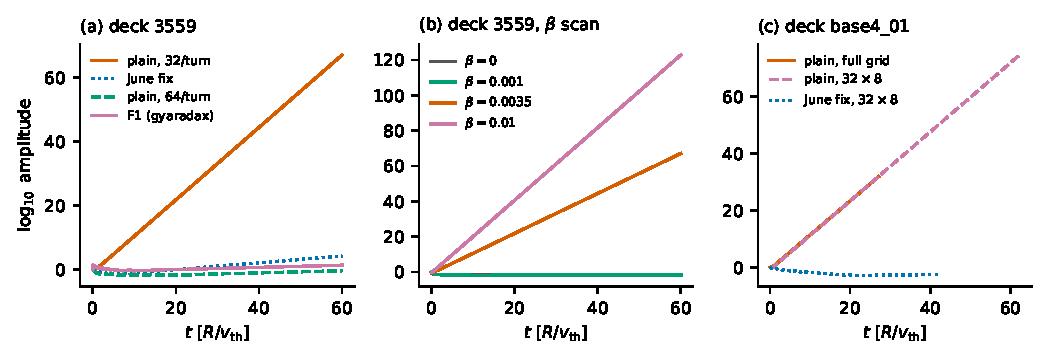
\includegraphics[width=\textwidth]{fig_blowup.pdf}
\caption{The instability in GKW develop, as $\log_{10}$ of the mode amplitude (time integral of the growth rate). (a) Deck 3559 as attached to the thread (32 points per turn), the same deck at 64 points per turn, the June fix (Section~4), and F1 (Section~6; gyaradax, since GKW has no F1). (b) Deck 3559 at 32 points per turn for four values of $\beta$. (c) Deck base4\_01 on its full grid ($48\times16$ velocity points) and on a reduced $32\times8$ grid, with and without the June fix.}
\label{fig:blowup}
\end{figure}

\begin{figure}[h]
\centering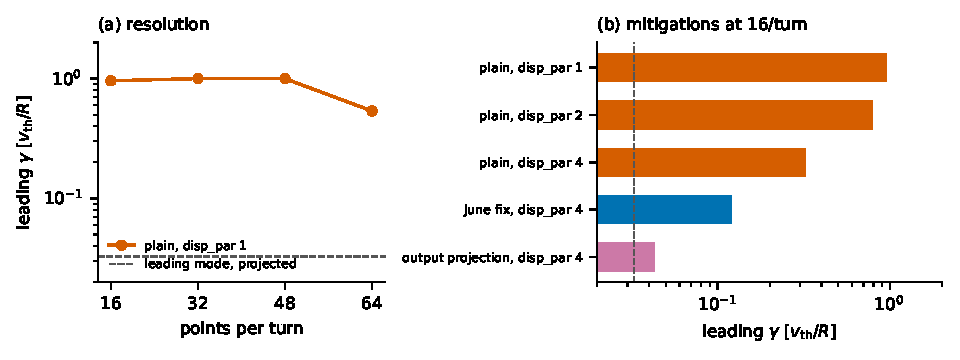
\includegraphics[width=0.95\textwidth]{fig_prod.pdf}
\caption{gyaradax eigenvalues on a production-type deck ($k_\theta\rho=0.05$, $\beta=0.005$, 21 turns, $32\times8$ velocity points, \code{disp\_vp}~0.2). (a) Leading growth rate against parallel resolution with plain dissipation (\code{disp\_par}~1). Dashed: the leading mode with the output-side projection (gyaradax mode 5, the per-species form of F1 plus the current projection). (b) At 16 points per turn: stronger dissipation, the June fix and the output-side projection.}
\label{fig:prod}
\end{figure}

\begin{figure}[h]
\centering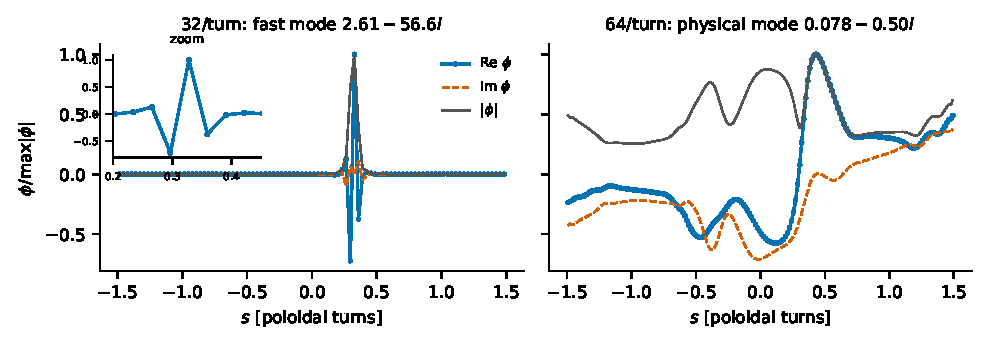
\includegraphics[width=\textwidth]{fig_structure.pdf}
\caption{Parallel structure of $\phi$ (GKW \code{parallel.dat}), normalised and phase-aligned at its maximum. Left: the fast mode at 32 points per turn, with a zoom on the grid-scale oscillation. Right: the physical mode at 64 points per turn on the deck's 3 turns. Its amplitude at the chain ends is not small: the physical mode is not converged in domain length (Section~1).}
\label{fig:structure}
\end{figure}

\section{Equations in GKW notation}

Per species $s$ with charge $Z_s$ (\code{signz}), density $n_s$ (\code{de}), temperature $T_s$ (\code{tmp}), thermal velocity ratio $v_{R,s}$ (\code{vthrat}) and Maxwellian $F_M$ (\code{fmaxwl}), GKW advances
\begin{equation}
g_s = f_s + \frac{2Z_s v_{R,s} v_\parallel}{T_s} J_0 A_\parallel F_M ,
\qquad
\frac{\partial g_s}{\partial t} = \mathcal{L}_s[f, \phi, A_\parallel] + \mathcal{D}_s[f_s].
\end{equation}
$\mathcal L$ holds Terms I to XI. The linear terms act on $f$ (\code{matg2f} in \code{exp\_integration.F90}). The discrete velocity integral at $(i_x, i_s)$ is
\begin{equation}
\vint{a} = \sum_{j,k} B_N\, \code{intmu}_j\, \code{intvp}_{i_s j k s}\, a_{jk},
\end{equation}
as in \code{poisson\_int}. The fields are
\begin{align}
\textstyle\sum_s Z_s n_s \vint{J_0 f_s} &= -\textstyle\sum_s \frac{Z_s^2 n_s}{T_s}\,(\Gamma_0(b_s) - 1)\,\phi \equiv \mathcal P\,\phi, \qquad \mathcal P > 0, \\
(k_\perp^2 + K)\, A_\parallel &= \beta \textstyle\sum_s Z_s n_s v_{R,s} \vint{J_0 v_\parallel g_s}, \qquad
K = \beta \textstyle\sum_s \frac{2 Z_s^2 n_s v_{R,s}^2}{T_s} \vint{v_\parallel^2 J_0^2 F_M}.
\label{eq:ampere}
\end{align}
The second form of Amp\`ere's law is the one GKW solves for $g$ (\code{ampere\_dia} holds $k_\perp^2 + K$). $K$ is the skin term. Electrons dominate it by the mass ratio, so $K \approx d_e^{-2}$ with $d_e$ the electron skin depth in units of $\rho_{\mathrm{ref}}$. The parallel dissipation (\code{parallel\_dissipation} in \code{linear\_terms.f90}) is
\begin{equation}
\mathcal D_s[f]_{i} = \code{disp\_par}\; c_s\, \frac{\code{ffun}_i\, v_{R,s}}{\Delta s} \sum_m w_m\, f_{i+m}, \qquad
w = \tfrac{1}{12}(-1, 4, -6, 4, -1).
\end{equation}
Here $c_s = |v_\parallel|$ for \code{idisp}~1 and $c_s = v_{\parallel,\mathrm{rms}}$ (\code{vpgr\_rms}) for \code{idisp}~2. Taps across $s$ boundaries follow \code{connect\_parallel}. The two points next to an open chain end use the one-sided rows of \code{differential\_scheme}. The odd-even mode is damped at $\tfrac{16}{12}\,\code{disp\_par}\, c_s\, \code{ffun}\, v_{R,s}/\Delta s$, about 60 times faster for electrons than for ions at \code{idisp}~2.

\section{Free energy and the source of the mode}

Define the weighted product and the free energy of one $k_y$ chain
\begin{equation}
\ip{a}{b} = \sum_s n_s \sum_{i} \Delta s\, \vint{\frac{T_s}{F_M}\, a^* b}, \qquad
W = \tfrac12\ip{f}{f} + \tfrac12 \mathrm{Re}(\phi^* \rho_f) + \tfrac12\mathrm{Re}(A_\parallel^* j_f).
\end{equation}
Here $\rho_f = \sum_s Z_s n_s \vint{J_0 f_s} = \mathcal P\phi$ and $j_f = 2\sum_s Z_s n_s v_{R,s}\vint{J_0 v_\parallel f_s} = 2k_\perp^2 A_\parallel/\beta$. Each term is non-negative. Using the two field equations and the $v_\parallel$ parity of the grid, for any right-hand side
\begin{equation}
\frac{dW}{dt} = \mathrm{Re}\,\ip{H}{\frac{\partial g}{\partial t}}, \qquad H_s = f_s + \frac{Z_s}{T_s} J_0 \phi F_M .
\end{equation}
The $A_\parallel$ terms cancel because $\ip{f}{(2Z v_R v_\parallel/T) J_0 F_M} = j_f^*$. The identity holds numerically to $10^{-11}$ on every eigenvector of the discrete operator. The dissipation contributes
\begin{equation}
\mathrm{Re}\,\ip{H}{\mathcal D f} = \underbrace{\mathrm{Re}\,\ip{f}{\mathcal D f}}_{\text{damping}} + \underbrace{\mathrm{Re}\,(\phi^* \rho_{\mathcal D})}_{\text{field work}}, \qquad
\rho_{\mathcal D} = \sum_s Z_s n_s \vint{J_0\, \mathcal D_s f_s}.
\label{eq:split}
\end{equation}
The first term is the intended damping. It is non-positive where the rows are symmetric and negative semi-definite in $\ip{\cdot}{\cdot}$; GKW's interior rows nearly are, its open-end rows are not. The second term is the work done on $\phi$ by the charge the dissipation creates, and it has no sign. The current moment of $\mathcal D$ does not appear, because its effects on $A_\parallel$ and on $f$ cancel inside $W$. With $B_\parallel$ on, the same algebra adds the work of the $J_1$ pressure moment of $\mathcal D f$; this is derived but not checked.

On the 3559 physics (5 turns, 24 points per turn, $8\times2$ velocity points) the leading fast mode $3.62 - 49.6i$ has these contributions to its growth rate:

\begin{center}\small
\begin{tabular}{lr}
\toprule
contribution & to $\gamma$ \\
\midrule
electron field work & $+6.87$ \\
ion field work & $-3.26$ \\
damping $\mathrm{Re}\ip{f}{\mathcal D f}$ & $-0.32$ \\
gradient drive & $+0.33$ \\
\bottomrule
\end{tabular}
\end{center}

Streaming and Term VII cancel. The mode carries 79\% of $W$ in $\phi$ and 20\% in $A_\parallel$. The picture:
\begin{itemize}
\item The dissipation removes electron gyrocentre density in phase with $\phi$. At the $k_\perp$ minimum $\mathcal P\propto k_\perp^2\rho^2$ is small, so $\phi$ responds strongly. The ion term has the opposite sign and is smaller by $v_{th,i}/v_{th,e}$. Weighting by $|v_\parallel|$ (\code{idisp}~1) makes it worse ($9.70$ against $3.62$).
\item $A_\parallel$ enables the mode but does not drive it. Below $\beta_c$ the electrons cancel the charge by streaming. Above it the skin term dominates $k_\perp^2$ at the minimum ($K \gg k_\perp^2$), the grid-scale oscillation becomes Alfv\'enic, and the charge accumulates. This is the property the skin gate of Section~8 uses.
\item Projections that remove only the current leave the mode unchanged. Every projection that removes the density removes it.
\item The same charge drives a mode on a closed loop with no ends and no gradients ($0.016 - 3.04i$ at 16 points per turn), so open ends are not the cause.
\item The time integrator and the field solve are not the cause: the mode is an eigenvalue of the space-discrete operator and does not move with the time step, and it does not move with the velocity resolution (2.608 and 2.654 at twice $n_{v_\parallel}$ and $n_\mu$). Both \code{idisp} options have it, and so does the scheme without dissipation ($0.22+244i$).
\end{itemize}

\section{The June fix}

The June 2026 fix (GKW branch \code{issue201-conservative-dissipation}, gyaradax \code{disp\_par\_conserve} modes 1 to 3) projects the input of the stencil:
\begin{equation}
\mathcal D^{\mathrm{June}}_s f = \mathcal D_s\!\left[f_s - J_0 F_M\frac{\vint{J_0 f_s}}{\vint{J_0^2F_M}} - J_0 v_\parallel F_M\frac{\vint{J_0 v_\parallel f_s}}{\vint{J_0^2v_\parallel^2F_M}}\right], \qquad 0 < k_\theta\rho \le \code{kycut}.
\end{equation}
It removes the fast mode on deck 3559 and on the ITER hybrid case of the thread ($2.79\to0.038$). It does not recover the physical mode. On deck 3559 it leaves $0.246 - 0.757i$, 3.3 times the physical $0.078 - 0.50i$ at 64 points per turn, and at 64 points per turn it still gives $0.26$ against $0.076$ plain (Figure~\ref{fig:blowup}, dotted). Two reasons:
\begin{itemize}
\item An input-side projection leaves the commutator of the stencil with $J_0(s)$ and, more importantly, the truncated open-end rows. Within 3 points of an open end 41--45\% of the $J_0$ density of the output survives, so the charge is not removed where the chain ends.
\item The projected input changes what the open-end rows act on, which changes the end condition and moves the physical mode by $O(1)$ on short chains.
\end{itemize}
The current projection does nothing for this mode (Section~3), and the \code{kycut} gate is a threshold in $k_y$ that changes results.

\section{What CGYRO does}

CGYRO's upwind dissipation acts on $|\xi| v\, f/F$ with a 6th-order filter and is projected per species at each $(\theta, k_x, n)$. Since commit eb8884c1 (August 2026) the projection is on the output side:
\begin{equation}
\mathcal D_C f = -\,\code{UP\_THETA}\,|\omega_{\mathrm{stream}}|\,(I - P_n - P_j)\, S\!\left[|\xi| v f/F\right],\quad
P_n x = J_0 \frac{\vint{J_0 x}}{\vint{J_0^2}},\quad
P_j x = J_0 v_\parallel \frac{\vint{J_0 v_\parallel x}}{\vint{J_0^2 v_\parallel^2}} .
\end{equation}
From 2016 until then (JCP 324 (2016) 73, eq.~88) the density, without $P_j$, was removed from the stencil input. The residual charge was then the commutator of the stencil with $J_0(\theta)$, which vanishes for electrons. Either way $\rho_{\mathcal D}\approx0$, so the field-work term in \eqref{eq:split} is absent. CGYRO chains are closed loops, so there are no open-end rows. The projection acts at every $\theta$ point and every $k_y$.

Figure~\ref{fig:cgyro} compares the two codes. On deck 3559, gyaradax with plain dissipation reproduces GKW's blowup; the June fix leaves $0.246$, and F1 settles at the physical level ($0.079$ against GKW's $0.078$ at 64 points per turn). CGYRO ran on a Miller-circle analogue of deck 3559 ($N_\theta=32$, $N_r=4$); its growth rates below are converted to GKW units.
\begin{itemize}
\item Both builds (before and after eb8884c1) settle to the physical mode ($0.112 - 0.363i$) and agree to three digits. So the current projection added in eb8884c1 is not what protects CGYRO.
\item With the projection removed (a two-line change to the pre-eb8884c1 build), CGYRO grows at $9.3$ and the run stops at $t\approx2$. The growth depends on $\beta$ like the GKW mode: $0.03$, $0.71$, $9.3$, $12.6$ and $16.0$ at $\beta = 10^{-4}$, $0.002$, $0.0035$, $0.005$ and $0.01$. It is $0.03$ electrostatically and is gone at $N_\theta \geq 64$.
\item With \code{UP\_THETA}~0 (no parallel dissipation) CGYRO grows too ($\approx5$). The dissipation-free centred scheme is not stable in either code.
\end{itemize}
The unprojected CGYRO mode has a different frequency and also appears at $\theta_0 = 0$, so it is not shown to be the same mode as GKW's. Both are explained by the same source: charge created by the dissipation.

\begin{figure}[h]
\centering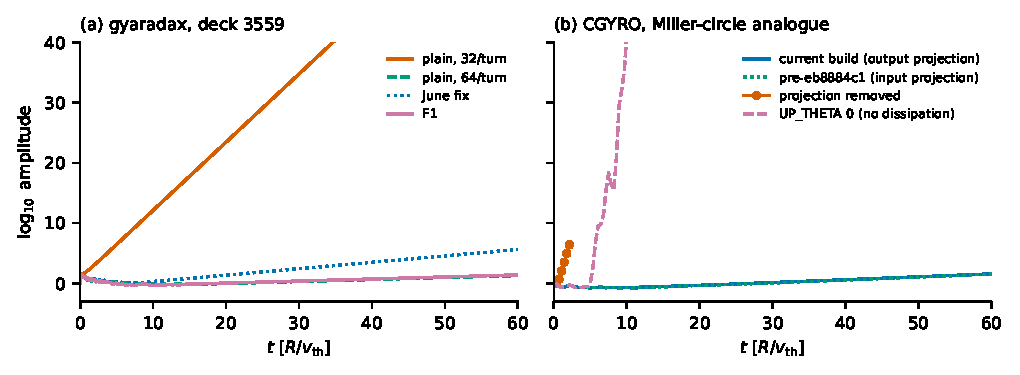
\includegraphics[width=\textwidth]{fig_cgyro.pdf}
\caption{$\log_{10}$ of the mode amplitude. (a) gyaradax on deck 3559, initial-value runs from noise (fp64): plain dissipation at 32 and 64 points per turn, the June fix (\code{disp\_par\_conserve}~2) and F1 (total charge, output side, \code{END}~3). (b) CGYRO on the Miller-circle analogue of deck 3559 ($\beta=0.0035$, $N_\theta=32$, $N_r=4$), converted to GKW units. The run without the projection stops at $t\approx2$.}
\label{fig:cgyro}
\end{figure}

\section{Projecting the charge everywhere: F1 and F2}

Let $u_s = (Z_s/T_s) J_0 F_M$, so that the gyro-averaged charge is $\rho[x] = \ip{u}{x}$ pointwise, and let $P x = u\,\rho[x]/\rho[u]$ be the total-charge projector at each $(s, k_x, k_y)$. Two output-side forms remove the charge of the dissipation:
\begin{align}
\mathcal D^{\mathrm{F1}} f &= (I-P)\,\mathcal D f, \label{eq:f1}\\
\mathcal D^{\mathrm{F2}} f &= \mathcal D f - P\,\mathcal D\,(I-P) f . \label{eq:f2}
\end{align}
Written out, F1 subtracts from $\mathcal D_s f_s$ the broadcast $u_s\,\rho_{\mathcal D}/\rho[u]$. It is the smallest change in the free-energy norm that makes $\rho_{\mathcal D}=0$. F2 removes only the charge made by dissipating the charge-free part of $f$. The two differ by $P\mathcal D P f$, the dissipation of the charge-carrying part, which F2 keeps: an odd-even charge is damped at the plain rate with F2 and not at all with F1. At the \code{END} points nearest an open chain end both keep the plain rows, which are GKW's boundary condition. The per-species variant of F1 (CGYRO's form without $P_j$) frees an odd-even mode in $s$ on electrostatic TEM cases ($0.240$ on R3 $n=4$, against $0.469$ for the TEM) and is not considered further.

With \eqref{eq:f1}, $\rho_{\mathcal D} = 0$ away from the ends and $\mathrm{Re}\,\ip{H}{\mathcal D^{\mathrm{F1}} f} = \mathrm{Re}\,\ip{(I-P) f}{\mathcal D f}$, which has no field-work term. F2 has no field-work term from the charge-free part either; what remains is of the sign of $\mathcal D$ up to the $s$-dependence of the polarisation.

\paragraph{Linear results.} Both forms remove the fast mode at every point tried and agree with each other to $10^{-4}$ on the electromagnetic production-type grids:

\begin{center}\small
\begin{tabular}{L{5.6cm}p{2.9cm}p{2.9cm}p{3.2cm}}
\toprule
case, grid & plain & F1 / F2 & reference \\
\midrule
3559 physics, 5 turns, 48 per turn & $0.1209-0.388i$ & $0.1202$ / $0.1198$ & \\
3559 physics, 5 turns, 24 per turn, \code{idisp} 1 & fast; $0.1021$ & $0.1005$ / not run & \\
i201, Miller circle, $(48, 64\times12)$, 31 turns ($c_s/a$) & fast $5.60$ & $0.0157+0.052i$ (both) & CGYRO $0.0148+0.0506i$ \\
Waltz $k_\theta\rho=0.05$, $\beta=0.005$, $(32,32\times12)$, 21 turns & numerical $0.43$--$0.49$ & $0.0207$ / $0.0206$ & CGYRO $0.022$--$0.024$ \\
R3 $n=4$, electrostatic, $(32,32\times12)$, 31 turns & $0.469$ & $0.4685$ / $0.4679$ & \\
\bottomrule
\end{tabular}
\end{center}

Figure~\ref{fig:spectra} shows the full spectrum on the 3559 physics. F1 removes the three fast modes and leaves the physical mode at $0.1207 - 0.396i$, against $0.1223 - 0.399i$ plain.

\begin{figure}[h]
\centering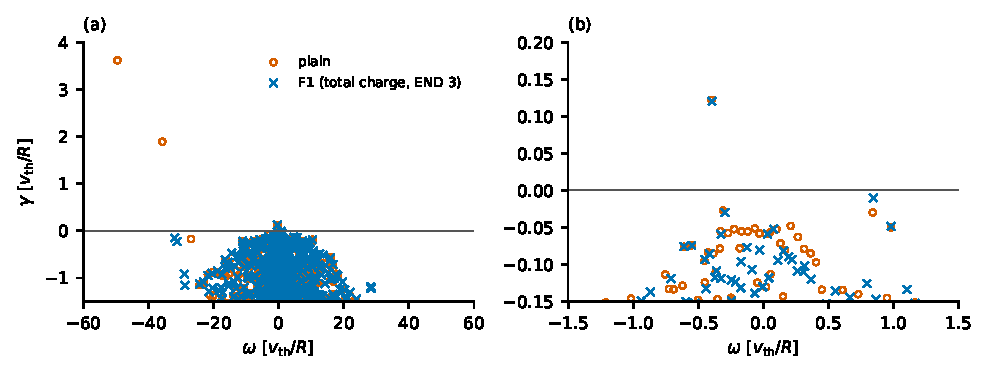
\includegraphics[width=\textwidth]{fig_spectra.pdf}
\caption{Complete spectra (3840 eigenvalues) of the linear operator on the 3559 physics: 5 open turns, 24 points per turn, $8\times2$ velocity points, \code{disp\_par} 2. (a) The fast modes $3.62-49.6i$ and $1.89-35.8i$ (plain) are absent with F1. (b) The physical mode is unchanged.}
\label{fig:spectra}
\end{figure}

\section{Why projecting everywhere fails}

\paragraph{Nonlinear results.} F2 was run on the four kinetic validation decks at their production grid ($2\times32\times12\times18\times192\times32$, 18 points per turn), option against plain with the same code, driver and GPU type, fluxes over the last 30\% of each run. These decks are electrostatic, so issue 201 does not occur on them; the test is whether the form leaves the physics alone.

\begin{center}\small
\begin{tabular}{L{4.2cm}p{1.2cm}p{4.6cm}p{4.6cm}}
\toprule
deck & $\hat s$ & F2 against plain & linear-phase growth, plain / F2 \\
\midrule
itg\_collisionless & 1.69 & $Q_i$ $+9.5\%\pm3.5\%$, $Q_e$ $+21.5\%\pm3.8\%$ & 0.145 / 0.142 \\
tem\_high\_flux & 0.28 & $Q_i$ $-20\%$, $Q_e$ $-18\%$, $\Gamma$ $-17\%$ & about equal \\
tem\_low\_flux & 2.67 & $Q_i$ $-72\%$, $Q_e$ $-54\%$, $\Gamma$ $-68\%$ & 0.151 / 0.076 \\
itg\_mid\_flux & 3.74 & not saturated by $t=350$ & 0.090 / 0.02--0.04 \\
\bottomrule
\end{tabular}
\end{center}

The spread of the plain controls against stored references is $-4.5\%$ to $+18\%$ in $Q_i$, so all but the itg\_collisionless ion flux are far outside it. With adiabatic electrons F2 is close to plain ($+1$ to $+2\%$ on a high-shear ITG case, $-8\%\pm3\%$ on a base ITG case, four realisations each); F1 lowers the high-shear flux by $25\%\pm3.5\%$ at 16 points per turn, because with one kinetic species it leaves the grid-scale density undamped. F2 was rejected on these results.

\paragraph{Mechanism: the physical modes contain the field work.} Single-turn chains of three validation decks at the production grid (18 points per turn, $32\times12$ velocity points, $\theta_0=0$), growth rate and the two dissipation terms of \eqref{eq:split} evaluated on the plain mode:

\begin{center}\small
\begin{tabular}{L{4.0cm}p{1.4cm}p{1.6cm}p{1.6cm}p{2.0cm}p{2.4cm}}
\toprule
deck ($\hat s$), $k\rho$ & collisions & plain & F2 & damping on plain mode & electron field work on plain mode \\
\midrule
tem\_low\_flux (2.67), 0.125 & off & $0.2655$ & $0.1848$ & $-0.336$ & $+0.232$ \\
 & on & $0.0593$ & $-0.0166$ & $-0.390$ & $+0.285$ \\
itg\_mid\_flux (3.74), 0.186 & off & $0.0101$ & $-0.1425$ & $-0.174$ & $+0.066$ \\
 & on & $0.0010$ & $-0.1592$ & $-0.173$ & $+0.064$ \\
itg\_collisionless (1.69), 0.195 & off & $0.0613$ & $0.0073$ & $-0.055$ & $+0.018$ \\
\bottomrule
\end{tabular}
\end{center}

At 18 points per turn the direct damping of the plain dissipation on these physical modes is as large as their growth rate, and 30 to 70\% of it comes back as work of $\phi$ on the electron charge the dissipation makes. That return is the term F1 and F2 remove by construction, so they overdamp the mode. The shift is the same with and without collisions, so collisions are not the cause. It is largest at high shear, where the mode ($\Delta\theta\sim1/\hat s = 0.27$~rad at $\hat s=3.7$) is narrower than the grid spacing (0.35~rad). F1 overdamps in the same way: on the same chains it gives $0.0193$ on itg\_collisionless (plain $0.0613$), $-0.0132$ on tem\_low\_flux with collisions (plain $0.0593$), loses the itg\_mid\_flux mode, and moves the two tem\_high\_flux modes by $+7\%$ and $-10\%$ (F2: $+5\%$, $-11\%$).

The conclusion is that no form which removes the field work at every point can keep the plain results at production resolution: at that resolution the plain growth rates contain it. CGYRO projects at every point and pays for it in the same way; on an adiabatic base ITG case its ion heat flux changes by 27\% between $N_\theta=16$ and 32. A remedy for issue 201 has to be confined to where the fast mode lives.

\paragraph{Other forms tried.} Applying the interior rows to $H$ instead of $f$ removes the field work with a sign-definite damping, but makes the operator stiff: the spectral radius on deck 3559 at 32 points per turn rises from 560 to 91045, which the explicit RK4 step cannot afford. A two-sided, provably dissipative form $(I-P)\mathcal D(I-P)$ lowers the physical mode by a factor 3 or more at 16 to 24 points per turn. The input-side June fix is discussed in Section~4.

\section{The skin-gated neutral dissipation}

\paragraph{Definition.} The fast mode lives where the skin term dominates $k_\perp^2$ in Amp\`ere's law \eqref{eq:ampere} (Section~3). Define at every $(s, k_x, k_y)$
\begin{equation}
\alpha_A = \frac{K}{k_\perp^2} \approx \frac{1}{(k_\perp d_e)^2},
\end{equation}
the inductive amplification of the electron response, and the gate $M = 1$ where $\alpha_A > \alpha_c$, $M=0$ elsewhere. The skin-gated neutral dissipation applies the F2 correction only inside the gate:
\begin{equation}
\mathcal D^{\mathrm{SG}} f = \mathcal D f - M\, P\,\mathcal D\,(I-P) f ,
\label{eq:sg}
\end{equation}
with the plain rows kept at the 4 points next to an open chain end. Outside the gate the dissipation is GKW's. $\alpha_c=100$ means the correction acts where $k_\perp d_e < 0.1$. The smooth gate replaces the step by
\begin{equation}
M = \frac{\alpha_A}{\alpha_A + \alpha_c},
\end{equation}
which is still zero without $A_\parallel$ but is non-zero at every point of an electromagnetic run.

Properties:
\begin{itemize}
\item Without $A_\parallel$, $K=0$ and the gate is empty. Electrostatic runs are bitwise the plain scheme; the implementation builds no tables for them.
\item With $A_\parallel$, $\alpha_A$ is large only near the $k_\perp$ minimum of low-$k_y$ chains at finite $\theta_0$, the points where the fast mode sits. Elsewhere the dissipation, including its field work on the physical modes, is unchanged.
\item There is one parameter, $\alpha_c$, with no cut in $k_y$, $\beta$ or resolution. It is a physical ratio, not a grid index.
\end{itemize}

\paragraph{Where it acts.} Number of gated points on the $k_y$ chain of each deck:

\begin{center}\small
\begin{tabular}{L{6.2cm}rrrrr}
\toprule
deck & max $\alpha_A$ & points & $\alpha_c=100$ & 300 & 1000 \\
\midrule
i201, 31 turns at 48 per turn & 1204 & 1488 & 23 & 10 & 2 \\
Waltz $k_\theta\rho=0.05$, $\beta=0.005$, 16 per turn & 7306 & 336 & 40 & 18 & 12 \\
Waltz $k_\theta\rho=0.1$, $\beta=0.005$ & 1838 & 992 & 34 & 24 & 12 \\
Waltz $k_\theta\rho=0.1$, $\beta=0.001$ & 368 & 992 & 20 & 8 & 0 \\
Waltz $k_\theta\rho=0.25$, $\beta=0.005$ & 294 & 992 & 18 & 0 & 0 \\
Waltz $k_\theta\rho=0.25$, $\beta=0.001$; $0.5$, $\beta=0.005$ & 59; 74 & 992 & 0 & 0 & 0 \\
R3, ITG, the four kinetic validation decks & electrostatic & & 0 & 0 & 0 \\
\bottomrule
\end{tabular}
\end{center}

\paragraph{Implementation.} The correction is F2's: one $J_0$-weighted moment of $f$, the plain stencil on the charge-free part, one more moment of its output and a broadcast with $u$, multiplied by the gate. In GKW it fits as a second pass in \code{calc\_linear\_terms}, with the gate read from \code{ampere\_dia} and $k_\perp^2$. In gyaradax it is an uncommitted worktree option (\code{solver.disp\_par\_neutral: true}, \code{disp\_par\_neutral\_end: 4}, \code{disp\_par\_neutral\_alpha:} $\alpha_c$; JAX backend). It costs one more parallel stencil in electromagnetic runs, about a factor 2 in the present JAX form on a B300; a fused kernel would be cheaper.

\section{Results on production grids}

fp64 Krylov eigen-solves in gyaradax. ``Fast'' is the largest growth among modes whose $\phi$ centroid along $s$ is above 0.3 of the Nyquist wavenumber.

\paragraph{The fast mode.}

\begin{center}\small
\begin{tabular}{L{4.3cm}p{2.0cm}p{1.9cm}p{1.9cm}p{1.9cm}p{1.9cm}}
\toprule
case, grid & plain & $\alpha_c=1000$ & 300 & 100 & 30 \\
\midrule
deck 3559, 32 per turn, $32\times8$ & $2.607$ & $0.78$ left & removed & removed & removed \\
i201, $(48,64\times12)$, 31 turns ($c_s/a$) & $5.60$ & removed & removed & removed & removed \\
base4\_01 reduced, $(36,32\times8)$, collisions off & $2.791$ & removed & removed & removed & removed \\
Waltz $k_\theta\rho=0.05$, 16 per turn & $0.376$ & $0.031$ left & removed & removed & removed \\
Waltz $k_\theta\rho=0.1$, $\beta=0.005$ (grid mode) & $0.212$ & removed & removed & removed & removed \\
\bottomrule
\end{tabular}
\end{center}

$\alpha_c$ between 30 and 300 removes the mode on every deck, a factor 3 to 10 below the largest value that still works on each. On coarse grids the margin at 300 is gone: an i201 chain at 16 points per turn (test grid, $32\times8$, \code{disp\_par}~1) kept a fast mode at 0.94 with $\alpha_c=300$. The base4\_01 deck runs without collisions, because gyaradax supports $Z_{\mathrm{eff}}=1$ only; its plain fast mode (2.791) matches GKW's.

\paragraph{The physical modes.} Growth-rate shift against the plain scheme on the same grid (``untouched'': no gated point, bitwise plain):

\begin{center}\small
\begin{tabular}{L{5.6cm}p{1.9cm}p{1.9cm}p{1.9cm}p{1.9cm}}
\toprule
case (plain value) & $\alpha_c=1000$ & 300 & 100 & 30 \\
\midrule
deck 3559, 32 per turn ($0.0756$) & & $+0.5\%$ & $+1.2\%$ & $+4.4\%$ \\
\quad against its 64-per-turn value ($0.0764$) & & $-0.5\%$ & $+0.1\%$ & $+3.3\%$ \\
i201 (CGYRO $0.0148+0.0506i$; $\omega$ 0.051 to 0.052 in every column) & $0.0158$ & $0.0155$ & $0.0156$ & $0.0156$ \\
base4\_01 reduced (marginal mode $-0.0001+0.259i$) & $-0.0003$ & $-0.0003$ & $-0.0003$ & $-0.0001$ \\
Waltz $k_\theta\rho=0.1$, $\beta=0.005$ ($0.0597-0.112i$) & $-5.1\%$ & $-1.5\%$ & $-0.1\%$ & $-0.6\%$ \\
Waltz $k_\theta\rho=0.1$, $\beta=0.001$ ($0.0744-0.056i$) & untouched & $+0.3\%$ & $+0.8\%$ & $-0.1\%$ \\
Waltz $k_\theta\rho=0.25$, $\beta=0.005$ ($0.1813-0.281i$) & untouched & untouched & $-1.9\%$ & $-0.1\%$ \\
Waltz $k_\theta\rho=0.25$, $\beta=0.001$ ($0.2398$) & untouched & untouched & untouched & $-0.02\%$ \\
R3, ITG, kinetic validation decks & untouched & untouched & untouched & untouched \\
\bottomrule
\end{tabular}
\end{center}

With $\alpha_c$ from 100 to 300 every physical mode on a production grid is within 2\%; the largest shifts are $-1.9\%$ (Waltz $k_\theta\rho=0.25$ at 100) and $-1.5\%$ (Waltz $k_\theta\rho=0.1$ at 300). No single value keeps every case within 1\%. The shift is not monotonic in $\alpha_c$: it depends on which few points fall just inside the hard edge of the gate. On 16-per-turn test grids the physical modes move by 6 to 27\%, where the plain value is itself 4 to 6\% off its resolved value.

\paragraph{Smooth gate and F1 inside the gate.} Worst shift in growth or frequency of the leading physical mode against the plain scheme on the same grid, 32 points per turn; the Waltz points are $k_\theta\rho$ 0.1, 0.25 and 0.5 at $\beta$ 0.001 and 0.005:

\begin{center}\small
\begin{tabular}{L{4.4cm}L{3.4cm}L{3.6cm}L{3.4cm}}
\toprule
form & worst, Waltz points & deck 3559, $\gamma$ / $\omega$ & fast mode \\
\midrule
step, $\alpha_c=300$ & $1.5\%$ & $+0.5\%$ / $-1.0\%$ & removed \\
step, $\alpha_c=100$ & $1.9\%$ & $+1.2\%$ / $-1.3\%$ & removed \\
step, $\alpha_c=30$ & $2.4\%$ & $+4.4\%$ / $-1.2\%$ & removed \\
smooth, $\alpha_c=300$ & $1.3\%$ & $+0.6\%$ / $-0.9\%$ & removed \\
smooth, $\alpha_c=100$ & $1.0\%$ & $+0.3\%$ / $-1.1\%$ & removed \\
smooth, $\alpha_c=30$ & $0.75\%$ & $+0.6\%$ / $-1.2\%$ & removed \\
smooth, $\alpha_c=1$ & $0.67\%$ & $+2.9\%$ / $-1.4\%$ & removed \\
F1 correction, step, $\alpha_c=100$ & $1.9\%$ & $+1.0\%$ / $-1.3\%$ & removed \\
\bottomrule
\end{tabular}
\end{center}

The smooth gate removes the fast mode on deck 3559, base4\_01, Waltz $k_\theta\rho=0.05$ and a 5-turn i201 chain; the 31-turn i201 solves were still running at the time of writing (every step gate passes there). Between $\alpha_c=30$ and 100 no Waltz value moves by more than 0.3\%. Inside the gate F1 and F2 agree within 0.15\%. The smooth gate touches every electromagnetic mode, where the step at 100 to 300 leaves Waltz $k_\theta\rho=0.5$ bitwise plain.

About 0.6\% is a floor for any weight in $s$: the smooth gate is an average of step results, and the physical modes carry the same term at the $k_\perp$ minimum as the fast mode, so no weight along $s$ separates them. Against the resolved plain value instead of the same-grid one, deck 3559 is at $-0.5$ to $+0.1\%$ in growth.

\paragraph{Against the remedies without a parameter.} Same cases, plain scheme:

\begin{center}\small
\begin{tabular}{L{2.6cm}p{4.0cm}p{4.0cm}p{4.0cm}}
\toprule
case & skin gate, $\alpha_c$ 100--300 & finer parallel grid & higher \code{disp\_par} \\
\midrule
deck 3559 & removed; $+0.5$ to $+1.2\%$ & removed at 64 per turn, about $4\times$ cost & removed at 4; physical $+12\%$ \\
i201 & removed; within 5\% of CGYRO & not removed up to 128 per turn & at 4 ($20\times$ the deck value) the leading mode changes \\
base4\_01 & removed; unchanged & removed at 108 per turn, about $9\times$ cost & removed at 8; time step $5\times$ smaller, $\omega$ $+5\%$ \\
Waltz $0.05$ & removed & not removed up to 64 per turn & not removed cleanly up to 8; $+18\%$ at 4 \\
electrostatic & untouched & nothing to do & nothing to do \\
\bottomrule
\end{tabular}
\end{center}

\section{Status of the evidence}

\paragraph{What is established.} The fast mode is driven by the field work of the dissipation's charge (a measured budget). Removing that charge everywhere removes the mode but changes physical results at production resolution, because the physical growth rates at 16 to 18 points per turn contain the same work (measured on three kinetic decks, F2). The skin gate removes the mode on deck 3559, i201, base4\_01 and the Waltz decks with $\alpha_c$ from 30 to 300, leaves electrostatic runs bitwise unchanged, and keeps physical eigenvalues on production grids within 2\% for $\alpha_c$ from 100 to 300.

\paragraph{What is not established.}
\begin{itemize}
\item \textbf{1\% tolerance.} The step gate reaches 2\%. The smooth gate at $\alpha_c$ 30 to 100 reaches 1\% on the Waltz points; deck 3559 stays at $-1.1$ to $-1.2\%$ in frequency against the same-grid plain value. 0.3\% is not reachable with any weight along $s$; it would need a correction that separates the modes in time (a high-pass of the removed charge, one extra state variable; untested).
\item \textbf{Coarse grids.} At 16 points per turn $\alpha_c=300$ has no margin and physical modes move by more than 5\%. On Waltz $k_\theta\rho=0.05$ at 16 points per turn every form puts the second physical mode at 0.013 to 0.015 against plain 0.0201 (resolved 0.0207); at 32 points per turn the forms give 0.0206 to 0.0208.
\item \textbf{base4\_01 with its collisions} has not been run ($Z_{\mathrm{eff}}>1$).
\item \textbf{Nonlinear.} First electromagnetic nonlinear runs on 27 November (Cyclone parameters, $\beta=0.005$, production grids): with kinetic electrons the plain scheme blows up by $t\approx1$ at the lowest $k_y$ and $\theta_0\approx\pm2.5$, both gates run; with adiabatic electrons the step gate at 300 is bitwise plain and the smooth gate at 100 changes $Q_i$ by $-1.4\%$, inside the scatter. See the handover README.
\end{itemize}

\clearpage
\appendix
\section{Configurations}
\label{app:configs}

The GKW decks 3559 and base4\_01 and the CGYRO analogue of deck 3559 come from the restricted issue bundle and are not reproduced here; their parameters are in Section~1 and in the handover README, and the files stay on the lab hosts.

\subsection*{The skin gate in gyaradax}
Worktree \code{gyaradax-f1}, uncommitted. Added to the \code{solver} section of a configuration:
\begin{lstlisting}
solver:
  disp_par_neutral: true
  disp_par_neutral_end: 4
  disp_par_neutral_alpha: 100.0
\end{lstlisting}

\end{document}
